\begin{figure}
	\centering
	\begin{tabular}{@{}cc@{}c@{}c@{}c@{}c@{}}
		\textbf{Frame} & \textbf{RGB} & \textbf{Depth} & \textbf{FORTH} & \textbf{Classification} & \textbf{3D Pose} \\ 
		\hline 
		\multicolumn{6}{c}{\textbf{Testing hand sequence $B$}} \\ 
		\hline 
		\raisebox{1.3cm}{\parbox{2cm}{\centering (a)\\Frame 303}} & 
		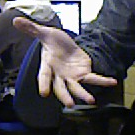
\includegraphics[width=2.35cm]{fig/hand/qual/rgb/image_0303.png} &
		
\includegraphics[width=2.35cm]{fig/hand/qual/depth/image_0303.png} &
		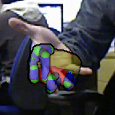
\includegraphics[width=2.35cm]{fig/hand/qual/forth/image_0303.png} &
		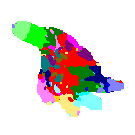
\includegraphics[width=2.35cm]{fig/hand/qual/class/class-303.png} &
		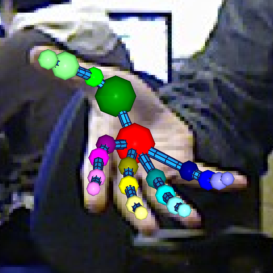
\includegraphics[width=2.35cm]{fig/hand/qual/vote/image_0303.png}
		\phantomsubcaption\label{fig/hand/multi1} \\
		\raisebox{1cm}{\parbox{2cm}{\centering (b)\\Frame 520}} & 
		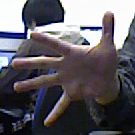
\includegraphics[width=2.35cm]{fig/hand/qual/rgb/image_0520.png} &
		
\includegraphics[width=2.35cm]{fig/hand/qual/depth/image_0520.png} &
		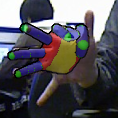
\includegraphics[width=2.35cm]{fig/hand/qual/forth/image_0520.png} &
		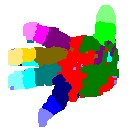
\includegraphics[width=2.35cm]{fig/hand/qual/class/class-520.png} &
		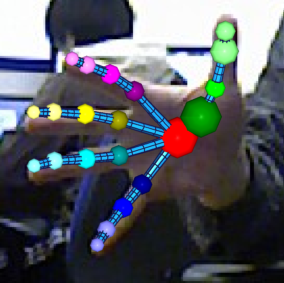
\includegraphics[width=2.35cm]{fig/hand/qual/vote/image_0520.png}
		\phantomsubcaption\label{fig/hand/multi2} \\
		\raisebox{1cm}{\parbox{2cm}{\centering (c)\\Frame 825}} & 
		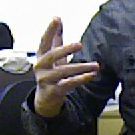
\includegraphics[width=2.35cm]{fig/hand/qual/rgb/image_0825.png} &
		
\includegraphics[width=2.35cm]{fig/hand/qual/depth/image_0825.png} &
		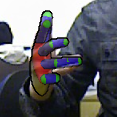
\includegraphics[width=2.35cm]{fig/hand/qual/forth/image_0825.png} &
		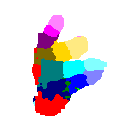
\includegraphics[width=2.35cm]{fig/hand/qual/class/class-825.png} &
		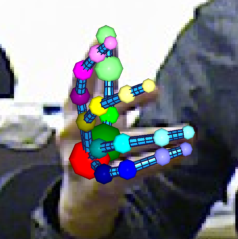
\includegraphics[width=2.35cm]{fig/hand/qual/vote/image_0825.png}
		\phantomsubcaption\label{fig/hand/multi3} \\
		\raisebox{1cm}{\parbox{2cm}{\centering (d)\\Frame 946}} & 
		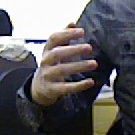
\includegraphics[width=2.35cm]{fig/hand/qual/rgb/image_0946.png} &
		
\includegraphics[width=2.35cm]{fig/hand/qual/depth/image_0946.png} &
		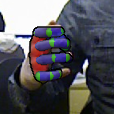
\includegraphics[width=2.35cm]{fig/hand/qual/forth/image_0946.png} &
		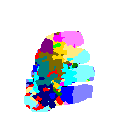
\includegraphics[width=2.35cm]{fig/hand/qual/class/class-946.png} &
		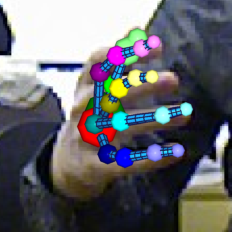
\includegraphics[width=2.35cm]{fig/hand/qual/vote/image_0946.png}
		\phantomsubcaption\label{fig/hand/multi4} \\
		\raisebox{1cm}{\parbox{2cm}{\centering (e)\\Frame 996}} & 
		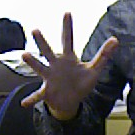
\includegraphics[width=2.35cm]{fig/hand/qual/rgb/image_0996.png} &
		
\includegraphics[width=2.35cm]{fig/hand/qual/depth/image_0996.png} &
		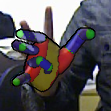
\includegraphics[width=2.35cm]{fig/hand/qual/forth/image_0996.png} &
		
\includegraphics[width=2.35cm]{fig/hand/qual/class/class-996.png} &
		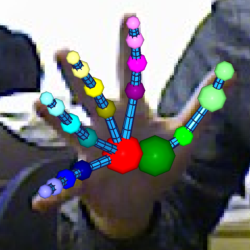
\includegraphics[width=2.35cm]{fig/hand/qual/vote/image_0996.png}
		\phantomsubcaption\label{fig/hand/multi5} \\ 
		\hline 
		\multicolumn{6}{c}{\textbf{Testing hand sequence $C$}} \\ 
		\hline 
		\raisebox{1cm}{\parbox{2cm}{\centering (f)\\Frame 198}} &
		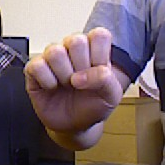
\includegraphics[width=2.35cm]{fig/hand/qual/rgb/image_0198.png} &
		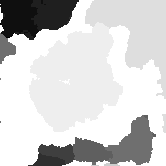
\includegraphics[width=2.35cm]{fig/hand/qual/depth/image_0198.png} &
		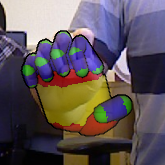
\includegraphics[width=2.35cm]{fig/hand/qual/forth/image_0198.png} &
		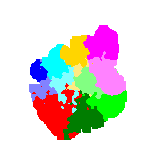
\includegraphics[width=2.35cm]{fig/hand/qual/class/class-198.png} &
		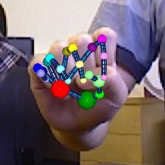
\includegraphics[width=2.35cm]{fig/hand/qual/vote/image_0198.png} 
		\phantomsubcaption\label{fig/hand/multi6} \\
		\raisebox{1cm}{\parbox{2cm}{\centering (g)\\Frame 440}} & 
		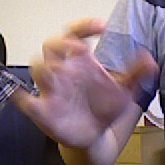
\includegraphics[width=2.35cm]{fig/hand/qual/rgb/image_0440.png} &
		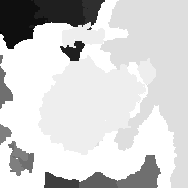
\includegraphics[width=2.35cm]{fig/hand/qual/depth/image_0440.png} &
		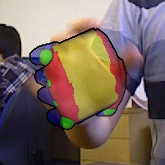
\includegraphics[width=2.35cm]{fig/hand/qual/forth/image_0440.png} &
		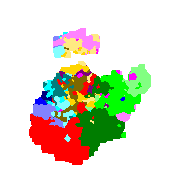
\includegraphics[width=2.35cm]{fig/hand/qual/class/class-440.png} &
		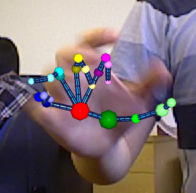
\includegraphics[width=2.35cm]{fig/hand/qual/vote/image_0440.png} 
		\phantomsubcaption\label{fig/hand/multi7} \\
	\end{tabular}
	\caption{\textbf{Qualitative experimental results of the multi-view experiment.} For each row, from left to right: RGB image, depth image, hand pose from FORTH, joint labels from the proposed method, final hand pose output of the proposed method.}
	\label{fig/hand/multiqual}
\end{figure} 
